\chapter{Introduction to Machine Learning}

Machine Learning can be defined as a software that automatically finds hidden patterns and connections in large datasets, without requiring a human expert to program every single rule. In a nutshell, ML is a process that aims to learn how to answer to questions based on data without rely to hard-coding algorithm.

\begin{figure}[h]
    \centering
    \includegraphics[width=0.35\linewidth]{images/chapter_1/chapter_1/Data_Science.png}
\end{figure}

\section{Big Data}

Big Data are Data which scale, diversity and complexity require new architectures, techniques, algorithms and analytics to manage it (due to huge volume), extract value and hidden knowledge from it.

Big Data can be generated by user content on the internet, log files, IoT and many other activities.

\subsection{5 Vs of Big Data}
Big Data is often characterized by 5 Vs:
\begin{itemize}
    \item \textbf{Volume:} Data volume increases exponentially over time. We reached the zettabytes of amount of data stored by the average company.
    \item \textbf{Velocity:} Speed at which this data is generated is fast. Fast data processing is needed to ensure timeliness.
    \item \textbf{Variety:} Various formats, types and structures of data.
    \item \textbf{Veracity:} Data quality may be compromised by misrepresenting data, data outliers, distorting and meaningless information. Therefore the accuracy, reliability and precision of data could be compromised.
    \item \textbf{Value:} translate data into business advantage, due to its usefulness in decision-making.
\end{itemize}

\section{Data Science}

Data Science is defined as the science that aims at extracting meaning from large quantities of data. Data Science follows a well-structured process:
\begin{itemize}
    \item \textbf{Data Generation and Data Acquisition}: Observation from real world generates Raw Data.
    \item \textbf{Selection}: Target data (raw data) is chosen in order to produce Clean Data.
    \item \textbf{Data Analysis}: Applying algorithms and statistical models to the data in order to extract meaning and find "Patterns".
    \item \textbf{Interpretation}: The final process of evaluating, summarizing, and communicating the found patterns to generate "Data Product".
    \item \textbf{Action}: Data Product can be used to decide or interact with real world.
\end{itemize}

\begin{figure}[h]
    \centering
    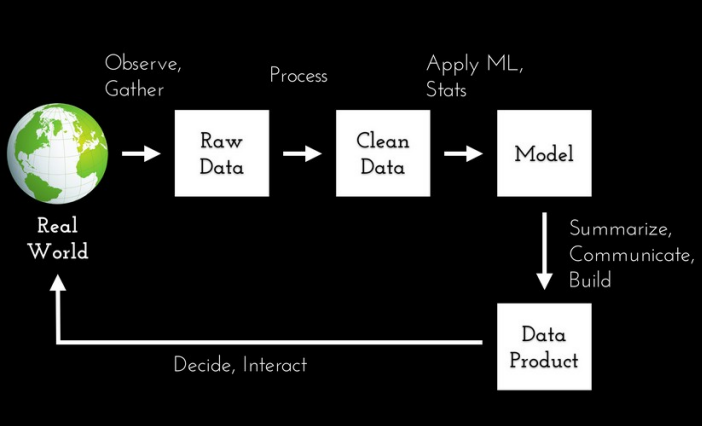
\includegraphics[width=0.5\linewidth]{images/chapter_1/Pipeline.png}
\end{figure}

In addition the Data Science Process is similar to the Knowledge Discovery in Databases (KDD).

\begin{figure}[h]
    \centering
    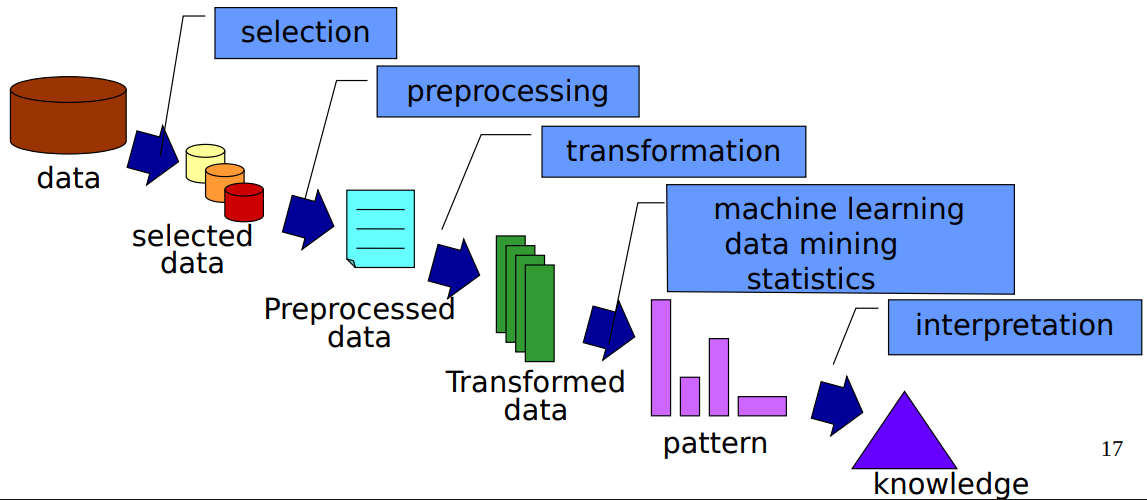
\includegraphics[width=0.5\linewidth]{images/chapter_1/Software_Pipeline.png}
\end{figure}

\subsection{Data Generation}
Data can be generated in different ways:
\begin{itemize}
    \item \textbf{Passive Recording:} log files, archives. Typically structured data.
    \item \textbf{Active Generation:} user-generated content, for instance social networks activity. Usually, semi-structured or unstructured data.
    \item \textbf{Automatic Production:} sensor-based IoT. It is location-aware, context-dependent and highly mobile data.
\end{itemize}

After the generation of data, Data Acquisition is required in order to Collect data. Transmit data to data centers and Prepocess it, in order to clean it, integrate and delete redundancies.

Data can be stored in Physical/Network Storage Infrastructures. The stored data needs then to be managed and processed by specific programming models.

\subsection{Data Preprocessing}
Real world data is considered as dirty and raw data. Without good quality data, no good quality pattern can be found. Therefore, the Data Preprocessing is needed in order to perform:
\begin{itemize}
    \item \textbf{Data Cleaning:} reducing noise effect, identifying or removing outliers and solve inconsistencies.
    \item \textbf{Data Integration:} reconciles data extracted from different sources, manages redundancy, identifies and solves data conflicts and integrates metadata.
\end{itemize}

\subsection{Data Analysis}
Data Analysis can be exploited in order to reach different objectives:
\begin{itemize}
    \item \textbf{Descriptive Analytics:} in order to know more about the data.
    \item \textbf{Predictive Analytics:} in order to take decision.
    \item \textbf{Prescriptive analytics:} in order to solve it in the future.
\end{itemize}

Different methods can be used to perform Data Analysis such as Machine Learning, data mining and statistical analysis.

It is important to note that Machine Learning and Data Mining share the common goal of extracting information from available data. Lastly, in the data science process defining the scope, techniques, evaluation of the process is advised.

\subsection{Artificial Intelligence}
ChatGPT, which is an AI language model, defines AI as the act of machines mimicking human intelligence to perform tasks. In a broader vision, the goals of AI research include reasoning, knowledge, representation, planning, learning, processing, perception, and support for robotics. To sum up, AI is the ability of a machine to imitate intelligent human behavior. Intelligence involves learning as AI Involves ML.

Therefore AI needs Machine Learning, in order to produce its intelligence.

\section{Machine Learning: Recap}

Machine Learning is all about fitting models to data in order to make predictions or forecasts.

It is important to note how Machine Learning is an application of AI. Additionally, Deep Learning is defined as an application of Machine Learning.

Inside Machine Learning, we will study the difference between Supervised and Unsupervised Learning.

\begin{figure}
    \centering
    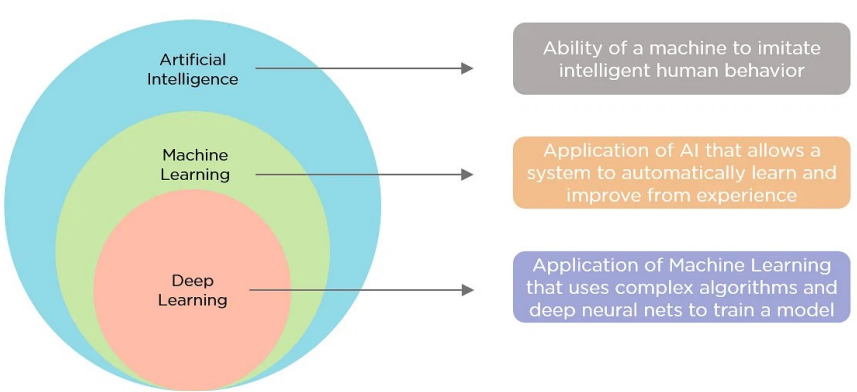
\includegraphics[width=0.5\linewidth]{images/chapter_1/ML_AI.png}
\end{figure}

To conclude, Machine Learning still faces some open issues such as the social impact derived from the interpretability and transparency of the analysis process in understandable terms to human beings. Other technical open issues are the scalability to huge data volumes, data dimensionality, data quality and the rise of heterogeneous data formats increasingly complex.


\section{A prova di coglione}
Il \textbf{Machine Learning (ML)} è un software che trova automaticamente pattern e relazioni nascosti in grandi dataset, \emph{imparando a rispondere a domande dai dati} senza che un esperto programmi ogni regola.

\paragraph*{Big Data.}
Sono dati la cui scala, diversità e complessità richiedono nuove architetture, tecniche e algoritmi per essere gestiti ed estrarne valore e conoscenza nascosta. Provengono da contenuti utente, file di log, IoT e molto altro, e si caratterizzano con le \textbf{5 V}:
\begin{itemize}
    \item \textbf{Volume}: crescita esponenziale (si è arrivati agli zettabyte);
    \item \textbf{Velocity}: generazione rapida, serve elaborazione veloce per restare tempestivi;
    \item \textbf{Variety}: formati, tipi e strutture diversi;
    \item \textbf{Veracity}: qualità a rischio (outlier, dati distorti o privi di senso), quindi accuratezza e affidabilità compromesse;
    \item \textbf{Value}: trasformare i dati in vantaggio di business, a supporto delle decisioni.
\end{itemize}

\paragraph*{Data Science.}
È la scienza che estrae significato da grandi quantità di dati, secondo un processo (simile al \textbf{KDD}) in cinque fasi: \textbf{generazione e acquisizione} (dal mondo reale ai \emph{raw data}) $\rightarrow$ \textbf{selezione} (i \emph{clean data}) $\rightarrow$ \textbf{analisi} (algoritmi e modelli statistici per trovare \emph{pattern}) $\rightarrow$ \textbf{interpretazione} (valutare, riassumere e comunicare i pattern, ottenendo il \emph{data product}) $\rightarrow$ \textbf{azione} (il data product serve a decidere o interagire con il mondo reale).

\paragraph*{Generazione e acquisizione.}
I dati nascono in tre modi: per \textbf{registrazione passiva} (log, archivi: dati strutturati), per \textbf{generazione attiva} (contenuti utente, social: semi- o non strutturati) o per \textbf{produzione automatica} (sensori IoT: dati contestuali, mobili e legati alla posizione). Segue l'\textbf{acquisizione}: raccolta, trasmissione ai data center e preprocessing (pulizia, integrazione, eliminazione delle ridondanze). I dati sono poi conservati in infrastrutture di storage fisiche o di rete e gestiti con appositi modelli di programmazione.

\paragraph*{Preprocessing.}
I dati reali sono sporchi e grezzi, e senza dati di qualità non si trovano pattern di qualità. Servono quindi:
\begin{itemize}
    \item \textbf{Cleaning}: ridurre il rumore, individuare o rimuovere gli outlier, risolvere le incoerenze;
    \item \textbf{Integration}: riconciliare dati da fonti diverse, gestire ridondanze e conflitti, integrare i metadati.
\end{itemize}

\paragraph*{Analisi dei dati.}
Persegue tre obiettivi: \textbf{descrittivo} (capire i dati), \textbf{predittivo} (prevedere per decidere) e \textbf{prescrittivo} (risolvere i problemi in futuro). Si usano ML, data mining e analisi statistica; ML e data mining condividono lo scopo di estrarre informazione dai dati. Conviene sempre definire in anticipo obiettivi, tecniche e valutazione del processo.

\paragraph*{Intelligenza Artificiale e ML.}
L'\textbf{AI} è la capacità di una macchina di imitare il comportamento intelligente umano (ragionamento, rappresentazione della conoscenza, pianificazione, apprendimento, elaborazione del linguaggio, percezione, robotica). Poiché l'intelligenza implica apprendimento, \textbf{l'AI ha bisogno del ML}. Il ML consiste nell'adattare modelli ai dati per fare previsioni; è un'applicazione dell'AI, e il \textbf{Deep Learning} è a sua volta un'applicazione del ML. Al suo interno si distingue tra apprendimento \textbf{supervisionato} e \textbf{non supervisionato}.

\paragraph*{Problemi aperti.}
L'impatto sociale, legato a \textbf{interpretabilità e trasparenza} del processo di analisi, che dovrebbe essere comprensibile all'uomo, e alcuni limiti tecnici: \textbf{scalabilità} a volumi enormi, \textbf{dimensionalità}, \textbf{qualità dei dati} e formati eterogenei sempre più complessi.